\documentclass{article}

\usepackage{fullpage}
\usepackage{url}
\usepackage{graphicx}
\usepackage{amsmath}
\usepackage{physics}
\usepackage{mathtools}
\usepackage{bbold}

\DeclareMathOperator{\erfi}{erfi}
\newcommand{\R}{\ensuremath{\mathbb{R}}}
\newcommand{\C}{\ensuremath{\mathbb{C}}}

\title{Quantum Mechanics I Excercise 6}
\author{Idan Stark}
\date{\today}

\begin{document}
\maketitle

\section{General Many-body Hamiltonian}
In this section we consider the Many-body Hamiltonian
\begin{equation}
    H = \sum_\alpha \epsilon_\alpha \hat{a}_\alpha^\dagger \hat{a}_\alpha + \frac{1}{2}\sum_{\alpha\beta\gamma\delta} V_{\alpha\beta\gamma\delta} \hat{a}_\alpha^\dagger \hat{a}_\beta^\dagger \hat{a}_\gamma \hat{a}_\delta
\end{equation}
Where the interaction matrix is non zero only for the cases $\alpha = \gamma$ and $\beta = \delta$ or $\alpha = \delta$ and $\beta = \gamma$. In other words, the Hamiltonian can be written as:
\begin{equation}
    H = \sum_\alpha \epsilon_\alpha \hat{a}_\alpha^\dagger \hat{a}_\alpha + \frac{1}{2}\sum_{\alpha\beta} V_{\alpha\beta} \hat{a}_\alpha^\dagger \hat{a}_\beta^\dagger \hat{a}_\alpha \hat{a}_\beta + \frac{1}{2}\sum_{\alpha\beta} U_{\alpha\beta} \hat{a}_\alpha^\dagger \hat{a}_\beta^\dagger \hat{a}_\beta \hat{a}_\alpha
\end{equation}
Where $V_{\alpha\beta} = V_{\alpha\beta\alpha\beta}$ and $U_{\alpha\beta} = V_{\alpha\beta\beta\alpha}$, without Einstien summation. Let us look at the interaction terms. Each of them can be split into two sums, $\alpha = \beta$ and $\alpha \ne \beta$. So, the Hamiltonian can be futher written as:
\begin{equation}
    H = \sum_\alpha \epsilon_\alpha \hat{a}_\alpha^\dagger \hat{a}_\alpha + \frac{1}{2}\left[\sum_{\alpha} \left(V_{\alpha\alpha} \hat{a}_\alpha^\dagger \hat{a}_\alpha^\dagger \hat{a}_\alpha \hat{a}_\alpha + U_{\alpha\alpha} \hat{a}_\alpha^\dagger \hat{a}_\alpha^\dagger \hat{a}_\alpha \hat{a}_\alpha\right) + \sum_{\alpha \ne \beta} \left(V_{\alpha\beta} \hat{a}_\alpha^\dagger \hat{a}_\beta^\dagger \hat{a}_\alpha \hat{a}_\beta + U_{\alpha\beta} \hat{a}_\alpha^\dagger \hat{a}_\beta^\dagger \hat{a}_\beta \hat{a}_\alpha\right)
    \right]
\end{equation}
The first interaction term can be written as
\begin{equation}
    \frac{1}{2}\sum_{\alpha} \left(V_{\alpha\alpha} \hat{a}_\alpha^\dagger \hat{a}_\alpha^\dagger \hat{a}_\alpha \hat{a}_\alpha + U_{\alpha\alpha} \hat{a}_\alpha^\dagger \hat{a}_\alpha^\dagger \hat{a}_\alpha \hat{a}_\alpha\right) = 
    \sum_{\alpha} \frac{V_{\alpha\alpha} + U_{\alpha\alpha}}{2}  \hat{a}_\alpha^\dagger \hat{a}_\alpha^\dagger \hat{a}_\alpha \hat{a}_\alpha 
\end{equation}
But since $\hat{a}_\alpha^\dagger \hat{a}_\alpha = \hat{n}_\alpha$, and $\hat{a}_\alpha^\dagger \hat{a}_\alpha = \hat{a}_\alpha \hat{a}_\alpha^\dagger - 1$:
\begin{equation}
    \hat{a}_\alpha^\dagger \hat{a}_\alpha^\dagger \hat{a}_\alpha \hat{a}_\alpha = 
    \hat{a}_\alpha^\dagger \hat{a}_\alpha \hat{a}_\alpha^\dagger \hat{a}_\alpha - \hat{a}_\alpha^\dagger \hat{a}_\alpha = \hat{n}_\alpha^2 - \hat{n}_\alpha
\end{equation}
Now let us notice that $V_{\alpha\alpha} = V_{\alpha\alpha\alpha\alpha} = U_{\alpha\alpha}$, so:
\begin{equation}
    \sum_{\alpha} \frac{V_{\alpha\alpha} + U_{\alpha\alpha}}{2}  \hat{a}_\alpha^\dagger \hat{a}_\alpha^\dagger \hat{a}_\alpha \hat{a}_\alpha =
    V_{\alpha\alpha} \left(\hat{n}_\alpha^2 - \hat{n}_\alpha\right)
\end{equation}
In the second interaction term, since $\alpha \ne \beta$, the operators with different indices commute, so:
\begin{equation}
    \frac{1}{2}\sum_{\alpha \ne \beta} \left(V_{\alpha\beta} \hat{a}_\alpha^\dagger \hat{a}_\beta^\dagger \hat{a}_\alpha \hat{a}_\beta + U_{\alpha\beta} \hat{a}_\alpha^\dagger \hat{a}_\beta^\dagger \hat{a}_\beta \hat{a}_\alpha\right) =
    \frac{V_{\alpha\beta} + U_{\alpha\beta}}{2}\hat{n}_\alpha \hat{n}_\beta
\end{equation}
So, naming $V_\alpha = V_{\alpha\alpha} = V_{\alpha\alpha\alpha\alpha}$ and $I_{\alpha\beta} = \frac{V_{\alpha\beta} + U_{\alpha\beta}}{2} = \frac{V_{\alpha\beta\alpha\beta} + V_{\alpha\beta\beta\alpha}}{2}$:
\begin{equation}
    H = \sum_\alpha \left[\left(\epsilon + V_{\alpha}\right) \hat{n}_\alpha + V_\alpha \hat{n}_\alpha^2\right] + \sum_{\alpha \ne \beta} I_{\alpha\beta} \hat{n}_\alpha a\hat{n}_\beta
\end{equation}
\subsection{Symmetries}
The above Hamiltonian preserves the number of particles in every mode $\hat{n}_\alpha$. This comes from $N$ $U(1)$ symmetries, one for each mode. The generators for these symmetries are $\hat{n}_\alpha$:
\begin{equation}
    \psi \rightarrow e^{i\theta \hat{n}_\alpha} \psi
\end{equation}
\subsection{Solution}
Since the Hamiltonian is diagonalizable in the number basis of each mode, the eigenfunctions can be written as a product of the $\hat{n}_\alpha$-particles functions:
\begin{equation}
    \ket{\Psi_{\{n_{\alpha}\}}} = \ket{n_1, n_2, \dots, n_N} = \prod_{\alpha} \left[a^\dagger_\alpha\right]^{n_\alpha}\ket{0}
\end{equation}
The Since each number operator $\hat{n}_\alpha$ on has the eigenvalue $n_\alpha$, this gives the spectrum:
\begin{equation}
    E_{\{n_\alpha\}} = \sum_\alpha \left[\left(\epsilon + V_{\alpha}\right) n_\alpha + V_\alpha n_\alpha^2\right] + \sum_{\alpha \ne \beta} I_{\alpha\beta} n_\alpha n_\beta
\end{equation}

\section{Born-Oppenheimer on a two-level model}
Let us consider the Hamiltonian
\begin{equation}
    H(P, Q) = H_0(P, Q) + h(Q)
\end{equation}
Where $P, Q$ change slow enough so that the Born-Oppenheimer approximation can be applied, and $h$ has two levels and can be approximated to a matrix similar to the Landau-Zener model:
\begin{equation}
    h(Q) = \begin{pmatrix}
        \epsilon & \Delta Q \\ \Delta Q & -\epsilon
    \end{pmatrix}
\end{equation}
Where $\Delta$ is a real constant.
\subsection{Finding the adiabadic basis}
Let us start by solving the "fast" part $h$ and find the adiabadic basis. It is defined as the solution to the eigenvalue problem:
\begin{equation}
    h(Q) \psi_n(Q) = E_n(Q) \psi_n(Q)
\end{equation}
The eigenvalues of $h$ are:
\begin{equation}
    \det
    \begin{vmatrix}
        \epsilon - E_n & \Delta Q \\ \Delta Q & -\epsilon - E_n
    \end{vmatrix} = E_n^2 - \epsilon^2 - \left(\Delta Q\right)^2 = 0
\end{equation}
\begin{equation}
    \epsilon_{\pm} = \pm \sqrt{\epsilon^2 + \left(\Delta Q\right)^2}
\end{equation}
Which makes the adiabadic basis:
\begin{equation}
    \phi_{\pm} = \frac{1}{\sqrt{2}}\begin{pmatrix}
        \text{sgn}(\Delta Q) \sqrt{1 + \eta_{\pm}}
        \\
        \pm \sqrt{1 - \eta_{\pm}}
    \end{pmatrix}
    \qquad
    \eta_{\pm} = \frac{\epsilon}{\epsilon_{\pm}}
\end{equation}
Figure \ref{fig:energy-levels} shows the adiabadic energy dependence on $\Delta Q$.
\begin{figure}[h]
    \centering
    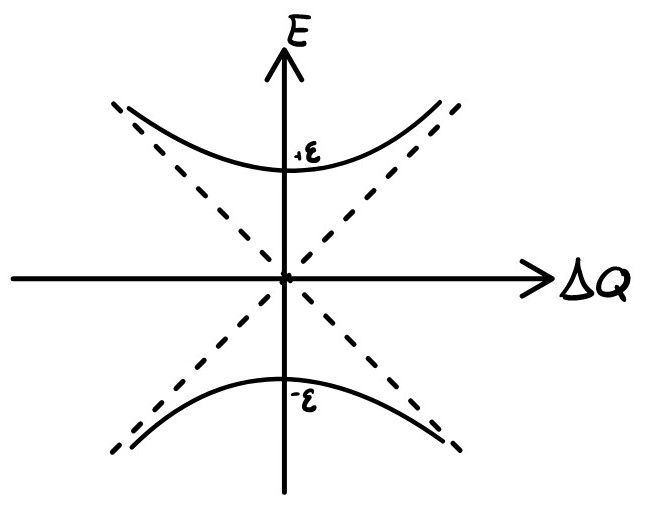
\includegraphics[width=0.6\textwidth]{energ-levels.jpg}
    \caption{Adiabadic energy levels $\epsilon_{\pm}$ as a function of $\Delta Q$}
    \label{fig:energy-levels}
\end{figure}
It can be seen that there is a level crossing at $Q = \epsilon = 0$.
\subsection{Berry phase}
The Berry phase is the phase induced by the geomatry of the energy levels:
\begin{equation}
    \gamma_{\pm} (t) = i \int_{Q_0}^{Q}\bra{\phi_{\pm}}\frac{\partial}{\partial Q'}\ket{\phi_{\pm}} dQ'
\end{equation}
But, for every pure real normalized wave function $\phi$, the matrix element $\bra{\phi_{\pm}}\frac{\partial}{\partial Q'}\ket{\phi_{\pm}} = 0$, and so the Berry phase is zero\footnote{The proof is shown in appendix 7.1 in the notes}.
\newline
This means we cannot count on it to tell us the positions of the level crossings. While for non-vanishing Berry phase, the Berry curvature has singularities at points in the parameter space where there is a level crossing, these singularities vanish when the Berry current $A_{\pm} = i\bra{\phi_{\pm}}\frac{\partial}{\partial Q'}\ket{\phi_{\pm}} = 0$. So even at the level crossing found at the previous section, the Berry current is zero.
\subsection{Born-Oppenheimer approximation}
Let us now consider the entire system with the Born-Oppenheimer approximated. Assuming
\begin{equation}
    H_0 = \frac{P^2}{2M} + U(Q)
\end{equation}
Where the potential energy $U(Q)$ has a minimum at some $Q_0$. Writing the wave function in the adiabadic basis $\phi_{\pm}$ with prefactors dependent on the slow changing coordinate $Q$:
\begin{equation}
    \psi(Q) = \xi_{+}(Q)\psi_{+} + \xi_{-}(Q)\psi_{-}
\end{equation}
The Born-Oppenheimer approximation then gives the equation
\begin{equation}
    \left(\frac{1}{2M}\left[-i\hbar \partial_Q - A_{\pm}\right]^2 + \left[U + \epsilon_{\pm}\right]\right)\xi_{\pm} = E \xi_{\pm}
\end{equation}
But since $A_{\pm} = 0$, these become:
\begin{equation}
\label{eq:BO}
    \left(-\frac{\hbar^2}{2M}\partial_Q^2 + U(Q) + \epsilon_{\pm}\right)\xi_{\pm} = E \xi_{\pm}
\end{equation}
This means the effective potential is
\begin{equation}
    U_{eff}^{(\pm)} = U(Q) + \epsilon_{\pm} = U(Q) \pm \sqrt{\epsilon^2 + \left(\Delta Q\right)^2}
\end{equation}
Taking $U(Q)$ to be symmetric around $Q_0$ with frequency $\omega$, we get:
\begin{equation}
    U_{eff}^{(\pm)} = U(Q) + \epsilon_{\pm} = \frac{1}{2}\omega(Q - Q_0)^2 \pm \sqrt{\epsilon^2 + \left(\Delta Q\right)^2}
\end{equation}
The two potential surfaces $U_{eff}^{(\pm)}$ can be seen in figure \ref{fig:effective-potential}.
\begin{figure}[h]
    \centering
    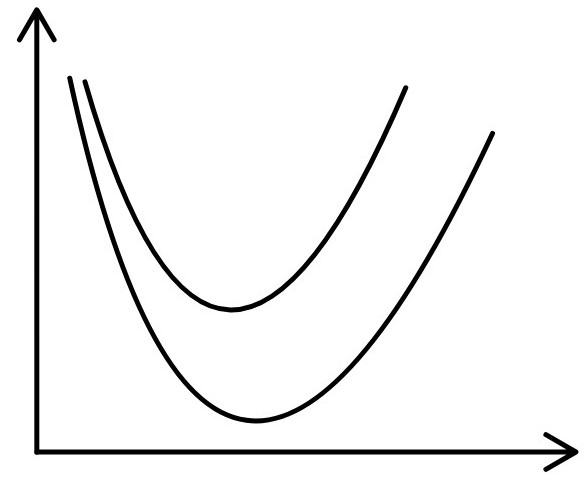
\includegraphics[width=0.6\textwidth]{u_eff.jpg}
    \caption{Effective potential surfaces $U_{eff}^{(\pm)}$ as a function of $Q$}
    \label{fig:effective-potential}
\end{figure}
These surfaces match a slightly assymteric well. Taking the Taylor expansion of $\epsilon_{\pm}$, we can approximate them to a second degree polynomial:
\begin{equation}
    U_{eff}^{(\pm)} \approx \frac{1}{2}\omega(Q - Q_0)^2 \pm \left[
        \epsilon_0 + \frac{\Delta^2 Q_0}{\epsilon_0}(Q - Q_0) + \frac{\epsilon^2\Delta^2}{2\epsilon_0^3}(Q - Q_0)^2
    \right]
    \qquad
    \epsilon_0 = \sqrt{\epsilon^2 + \left(\Delta Q_0\right)^2}
\end{equation}
Reogranizing we get a quadratic term:
\begin{equation}
    U_{eff}^{(\pm)} = \left(\frac{1}{2}\omega
    \pm \frac{\epsilon^2\Delta^2}{\epsilon_0^3}\right)(Q - Q_0)^2
    \pm \frac{\Delta^2 Q_0}{2\epsilon_0}(Q - Q_0)
    \pm \epsilon_0
\end{equation}
With a minimum point at:
\begin{equation}
    Q_{\min}^{(\pm)} = Q_0 \mp \tilde{Q}_{\pm}
    \qquad
    \tilde{Q}_{\pm} = \frac{\Delta^2\epsilon_0^2 Q_0}{2\omega\epsilon_0^3
    \pm 4\Delta^2\epsilon^2}
\end{equation}
 This is now a harmonic potential, and so we expect the energy levels to be close to those of the harmonic oscilator. We can find them using the WKB approximation. First, let us write $\xi_{\pm}$ as an exponent of some generally complex function $S(Q)$:
\begin{equation}
    \xi_{\pm}(Q) = \exp[-i\frac{S_{\pm}(Q)}{\hbar}]
\end{equation}
Then, pluggin it into equation \ref{eq:BO}:
\begin{equation}
    \left(-\frac{\hbar^2}{2M}\left[-i\frac{1}{\hbar}S_{\pm}'' - \frac{1}{\hbar^2}S_{\pm}'^2\right] + U_{eff}^{(\pm)} - E\right) = 0
\end{equation}
Openning up and taking $\hbar = 0$, we get:
\begin{equation}
    \frac{1}{2M}S_{\pm}'^2 + U_{eff}^{(\pm)} - E = 0
\end{equation}
Solving for $S_{\pm}'$:
\begin{equation}
    S_{\pm}' = \sqrt{2M\left(E - U_{eff}^{(\pm)}\right)}
\end{equation}
Which is the standard WKB result:
\begin{equation}
    S_{\pm}(Q) = \int \sqrt{2M\left(E - U_{eff}^{(\pm)}\right)} dQ
\end{equation}
Using the approximated effective potential, this is an integral of a 2nd-degree polynomial, which can be written around the minimum as:
\begin{equation}
\begin{gathered}
    U_{eff}^{(\pm)}(Q) \approx \alpha_{\pm}(Q - Q_{min}^{(\pm)})^2 + U_{eff, min}^{(\pm)}
    \\ \\
    \alpha_{\pm} = {U_{eff}^{(\pm)}}'' = \frac{1}{2}\omega
    \pm \frac{\epsilon^2\Delta^2}{\epsilon_0^3}\
    \qquad
    U_{eff,min}^{(\pm)} = U_{eff}^{(\pm)}(Q_{\min}^{\pm})
\end{gathered}
\end{equation}
And so the integral is
\begin{equation}
    S_{\pm}(Q) = \int \sqrt{2M\left(E - U_{eff, min}^{(\pm)}\right) - 2M\alpha_{\pm}\left(Q - Q_{min}^{(\pm)}\right)^2} dQ
\end{equation}
The solution to which is \footnote{It is extremely unfair that this theory took hold of the $\Delta$ sign, now all my difference variables look like variations.}
\begin{equation}
\begin{gathered}
    S_{\pm}(Q) = \delta E\sqrt{\frac{M}{2\alpha_{\pm}}}\arcsin\left(\sqrt{\frac{\alpha_{\pm}}{\delta E}}\delta Q\right) - \sqrt{\frac{M}{2\alpha_{\pm}}\left[\delta E - \alpha_{\pm}\delta Q^2\right]}\delta Q
    \\ \\
    \delta E = E - U_{eff, min}^{(\pm)}
    \qquad
    \delta Q = Q - Q_{min}^{(\pm)}
\end{gathered}
\end{equation}
The turning points are exactly where $\delta Q = \pm \sqrt{\delta E}$, so preforming the integral between them using the Bohr-Sommerfeld quantization condition:
\begin{equation}
    \oint S_{\pm}(Q) dQ = 2\pi \hbar \left(n + \frac{1}{2}\right)
\end{equation}
We get:
\begin{equation}
    \int_{-\sqrt{\delta E}}^{+\sqrt{\delta E}} \sqrt{2M\left(E - U_{eff}^{(\pm)}\right)} d\delta Q = 2\pi \hbar \left(n + \frac{1}{2}\right)
\end{equation}
Using the solution for $S_{\pm}(Q)$, this gives:
\begin{equation}
    \pi \delta E \sqrt{\frac{M}{2\alpha_{\pm}}} = 2\pi \hbar \left(n + \frac{1}{2}\right)
\end{equation}
So the energy levels are:
\begin{equation}
    E_n^{(\pm)} = \hbar \sqrt{\frac{2\alpha_{\pm}}{M}}\left(n + \frac{1}{2}\right) + U_{eff, min}^{(\pm)}
\end{equation}
\subsection{Summary}
Using the Born-Oppenheimer approximation for a two-level Landau-Zener like model, we manged to find two energy surfaces. We then used WKB to find countable infinity of energy levels on each of these surfaces. These energy levels can be seen in figure \ref{fig:energy-levels-full}. We can notice that the energy levels of the lower surface are closer to each other than those of the upper surface. This comes from the fact that $\alpha_{-} < \alpha_{+}$, which makes the frequency of the harmonic oscilator on the lower surface smaller than that of the upper surface.
\begin{figure}[h]
    \centering
    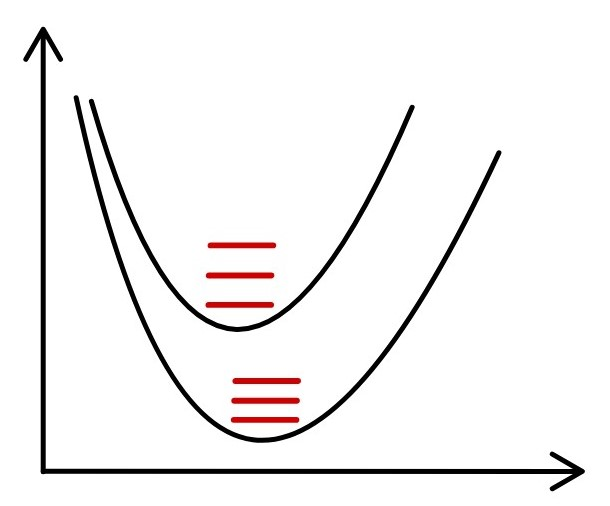
\includegraphics[width=0.6\textwidth]{u_eff_energy_levels.jpg}
    \caption{Full energy levels $E_n^{(\pm)}$}
    \label{fig:energy-levels-full}
\end{figure}
\end{document}